\documentclass[border=20pt]{standalone}
\usepackage{tikz}
\usepackage{amsmath}
\usetikzlibrary{calc,arrows.meta,angles,quotes}
\begin{document}
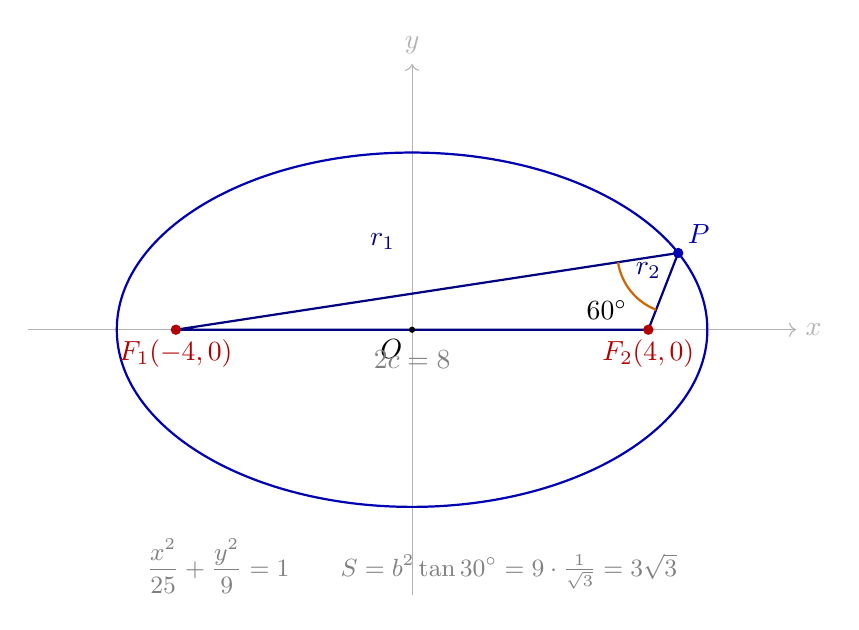
\begin{tikzpicture}[scale=0.75]
  % Axes
  \draw[->, gray!60, thin] (-6.5,0) -- (6.5,0) node[right] {$x$};
  \draw[->, gray!60, thin] (0,-4.5) -- (0,4.5) node[above] {$y$};

  % Ellipse: x^2/25 + y^2/9 = 1, a=5, b=3, c=4
  \draw[thick, blue!70!black] (0,0) ellipse (5 and 3);

  % Foci: F1(-4,0), F2(4,0)
  \coordinate (F1) at (-4, 0);
  \coordinate (F2) at (4, 0);
  \coordinate (O)  at (0,0);

  % P where ∠F1PF2 = 60° in ellipse x^2/25+y^2/9=1:
  % y_P = S / c = b^2·tan30° / c = 9·(1/√3) / 4 = 3√3/4 ≈ 1.299
  % x_P = a·√(1 - y_P²/b²) = 5·√(1 - 27/144) = 5·√(13/16) ≈ 4.506
  \coordinate (P) at (4.506, 1.299);

  % Triangle F1-P-F2
  \draw[thick, blue!50!black] (F1) -- (P) -- (F2) -- cycle;

  % 60° angle at P
  \draw pic["$60^\circ$", draw=orange!80!black, thick, angle eccentricity=1.5, angle radius=22] {angle=F1--P--F2};

  % Points
  \fill[red!70!black]  (F1) circle (2.5pt) node[below] {$F_1(-4,0)$};
  \fill[red!70!black]  (F2) circle (2.5pt) node[below] {$F_2(4,0)$};
  \fill[blue!70!black] (P)  circle (2.5pt) node[above right] {$P$};
  \fill[black]         (O)  circle (1.5pt) node[below left]  {$O$};

  % Labels
  \node[blue!50!black] at (-0.5, 1.5) {$r_1$};
  \node[blue!50!black] at (4.0, 1.0)  {$r_2$};
  \node[gray] at (0, -0.5) {$2c=8$};

  \node[text=gray, font=\small] at (0, -4.0)
    {$\dfrac{x^2}{25}+\dfrac{y^2}{9}=1\qquad S=b^2\tan30^\circ=9\cdot\frac{1}{\sqrt3}=3\sqrt3$};
\end{tikzpicture}
\end{document}
